\documentclass[12pt]{article} 

\usepackage{geometry}
\geometry{a4paper} 

\usepackage{graphicx} 
\usepackage{enumitem}
\usepackage{booktabs}

\usepackage{float} 
\usepackage{wrapfig} 

\usepackage{amsmath}
\usepackage{amsfonts}
\usepackage{amssymb}
\usepackage{dsfont}

\usepackage{tabularx}

\usepackage{xcolor}
\usepackage{listings}
\usepackage{caption}
\DeclareCaptionFont{white}{\color{white}}
\DeclareCaptionFormat{listing}{%
  \parbox{\textwidth}{\colorbox{gray}{\parbox{\textwidth}{#1#2#3}}\vskip-2pt}}
\captionsetup[lstlisting]{format=listing,labelfont=white,textfont=white}
\lstset{frame=lrb,xleftmargin=\fboxsep,xrightmargin=-\fboxsep}


\linespread{1.2} 
\setlength{\parskip}{\baselineskip} % vertical spaces
\setlength\parindent{0pt} % remove all indentation from paragraphs




\begin{document}

\title{\textbf{Model Adequacy Checking}}
\author{Hyunwoo Gu}
\date{}

\maketitle


%----------------------------------------------------------------------------------------
%	Section 1
%----------------------------------------------------------------------------------------
\section{Introduction}

Thus far the major \textbf{assumptions} that have been made as follows:

\begin{itemize}
  \item Relationship between $y$ and the regressors is linear, at least approximately
  \item Errors $\overset{\text{uncorr}}{\sim} (0, \sigma^2_{\text{constant}})$ 
  \item Errors $\overset{iid}{\sim} Normal$
\end{itemize}

We should always consider the adequacy of the model we have tentatively 

%----------------------------------------------------------------------------------------
%	Section 2
%----------------------------------------------------------------------------------------
\section{Residual Analysis}

\subsection{Definition of Residuals}

Residuals are defined by

$$
e_i := y_i - \hat{y}_i
$$

which may be viewed as the \textbf{deviation} between the \textbf{data} and the \textbf{fit}, and the variability in the response variable not explained by the regression model. It is convenient to think of the residuals as the \textbf{realized model errors}. Analysis of the residuals is an effective way to discover several types of model inadequacies. 

Residuals have zero mean, and their approximate average variance is estimated by

$$
\frac{\sum (e_i - \bar{e})^2}{n-p} = \frac{\sum e_i^2}{n-p} = MS_{Res}
$$


\subsection{Methods for Scaling Residuals}

\subsubsection*{Standardized Residuals}

Since the approximate average variance of a residual is estimated by $MS_{Res}$, a logical scaling for the residuals would be the \textbf{standardized residuals},

$$
d_i = \frac{e_i}{\sqrt{MS_{Res}}}
$$

The standardized residuals have mean zero and approximately unit variance. Thus, a large standardized residual potentially indicates an outlier.


\subsubsection*{Studentized Residuals}

Using $MS_{Res}$ as the variance of the $i$th residual, $e_i$ is only an approximation. We can improve the residual scaling by deviding $e_i$ by the exact standard deviation of the $t$th residual. 

$$
\begin{aligned}
e &= (I - H)y = X\beta - HX\beta + (I-H)\epsilon = (I-H)\epsilon\\[10pt]
\mathrm{Var}(e) &= \mathrm{Var}[(I-H) \epsilon] = \sigma^2 (I-H)
\end{aligned}
$$


Let $y_n$ be the observed response for the $n$th data point, $x_n$ the specific values for the regressors for this data point, $\hat{y}_n^\ast$ the predicted value for the response based on the other $n-1$ data points, $\delta=y_n - \hat{y}_n^\ast$ the difference between the actually observed value for this response compared to the predicted value based on the other values. 

If a data point is remote in terms of the regressor values and $|\delta|$ is large, then we have an influential point. Note that 

$$
\hat{y}_n = \hat{y}_n^\ast + h_{nn} \delta 
$$



$$
\begin{aligned}
\hat{y}_n &= \hat{y}_n^\ast + h_{nn} \delta \\[8pt]
&= 
\end{aligned}
$$


\subsubsection*{PRESS Residuals}

If we delete the $i$th observation, fit the regression model to the remaining $n-1$ observations, and calculate the predicted value of $y_i$ correspondoning to the deleted observation, the corresponding \textbf{prediction error} is 

$$
e_{(i)} = y_i - \hat{y}_{(i)}
$$

which is called \textbf{PRESS residuals} or \textbf{deleted residuals}. It turns out that $i$th PRESS residual is

$$
e_{(i)} = \frac{e_i}{1-h_{ii}}
$$



\subsubsection*{R-Student}





%--------------------------------
\subsection{Residual Plots}

We often plot externally studentized residuals \textbf{because they have constant variance}. 

\subsubsection*{Normal Probability Plot}
Gross nonnormality is potentially more serious as the $t$ and $F$ statistics and confidence and prediction intervals depend on the normality assumption. 


\subsubsection*{Plot of Residuals against Fitted Values $\hat{y}_i$}
A  plot of the residuals(preferrably the externally studentized residuals, $t_i$) versus the corresponding fitted values $\hat{y}_i$ is useful for detecting several common type of model inadequacies. The residuals should be plotted versus the fitted values $\hat{y}_i$, and not the observed values $y_i$, because the $e_i$ and $\hat{y}_i$ are uncorrelated while the $e_i$ and the $y_i$ are usually correlated. 

\textbf{Outward-opening funeel pattern} implies that the variance is an increasing function of 


\subsubsection*{Plot of Residuals against the Regressor}


\subsubsection*{Plot of Residuals in Time Sequence}. 
The time sequence plot of residuals may indicate that the errors at one time period are correlated with those at other time periods. The correlation between model errors at different time periods is called \textbf{autocorrelation}. 


%--------------------------------
\subsection{Partial Regression and Partial Residual Plots}




\textbf{Some Comments on Partial Regression Plots}. 

\textbf{Partial Residual Plots}. 

%--------------------------------
\setcounter{subsection}{5}
\subsection{Other Residual PLotting and Analysis Methods}


%----------------------------------------------------------------------------------------
% Section 3
%----------------------------------------------------------------------------------------
\section{PRESS Statistic}

The PRESS is generally regarded as a measure of how well a regression model will perform in \textbf{predicting new data}. A model with a small value of PRESS is desired.

$$
\begin{aligned}
\mathrm{PRESS} &= \sum_i^n [y_i - \hat{y}_{(i)}]^2 \\[8pt]
&= \sum_i^n \left( \frac{e_i}{1-h_{ii}} \right)^2
\end{aligned}
$$

\textbf{$R^2$ for Prediction Based on PRESS}. PRESS statistic can be used to compute an $R^2$-like statistic for prediction, 

$$
R^2_{prediction} = 1 - \frac{PRESS}{SS_T}
$$

which gives some indication of the \textbf{predictive capability} of the regression model. One very important use of the PRESS statistic is in \textbf{Comparing Models}. 


%----------------------------------------------------------------------------------------
%	Section 4
%----------------------------------------------------------------------------------------
\section{Detection and Treatment of Outliers}

An outlier is an extreme observation that is considerably different from the majority of the data. It is a data point that is not typical of the rest of the data. 

Residual plots against $\hat{y}_i$ and the normal probability plot are helpful in identifying outliers. Examining \textbf{scaled residuals}, such as the studentized and $R$-student residuals, is an excellent way to identify potential outliers. 

The effect of outliers on the regression model may be easily checked by dropping these points and refitting the regression equation. 



%----------------------------------------------------------------------------------------
%	Section 5
%----------------------------------------------------------------------------------------
\section{Lack of Fit of the Regression Model}

In the process of the wrong fitting, what we claim to be random error is actually a systematic departure as the result of not fitting enough terms. 

\subsection{A Formal Test for Lack of Fit}

The formal test for the lack of fit of a regression model assumes that the \textbf{normality}, \textbf{independence}, \textbf{constant-variance} requirements are met and that only the \textbf{first-order} character of the relationship is in doubt. 

The lack-of-fit test requires that we have replicate observations on the response $y$ for at least one level of $x$, which should be \textbf{true replications}, not just duplicate readings or measurements of $y$. The error variance $\sigma^2$ includes the measurement error and the variability associated with reaching the same level in different experiments. These replicated observations are used to obtain a \textbf{model-independent estimate} of $\sigma^2$. 

$$
\begin{aligned}
SS_{Res} &= SS_{PE} + SS_{LOF} \\[8pt]
\sum_i^m \sum_j^{n_i} (y_{ij} - \hat{y}_i)^2 &= \sum_i^m \sum_j^{n_i} (y_{ij} - \bar{y}_i)^2 + \sum_i^m n_i (\hat{y}_i - \hat{y}_i)^2
\end{aligned}
$$

If the assumption of constant variance is satisfied, $\sum_i^m \sum_j^{n_i} (y_{ij} - \bar{y}_i)^2$ is a \textbf{model-independent measure of pure error}, since only the variability of the $y$'s at each $x$ level is used to compute $SS_{PE}$, with the degree of freedom $\sum_i^m (n_i - 1) = n - m$.

$\sum_i^m n_i (\hat{y}_i - \hat{y}_i)^2$ is a weighted sum of squared deviations between the mean response $\bar{y}_i$ at each $x$ level and the corresponding fitted value. If the fitted $\hat{y}_i$ are close to the corresponding average responses $\bar{y}_i$, then there is a strong indication that the regression function is linear.



\subsection{Estimation of Pure Error from Near Neighbors}

A method is suggested for obtaining a model-independent estimate of error when there are no exact repeat points. These procedures search for points in $x$ space that are \textbf{near neighbors}, i.e., the sets of observations that have been taken with nearly identical levels of $x_1, \cdots, x_k$. As a measure of the distance between any two points, $x_{i1}, \cdots, x_{ik}$ and $x_{i'1}, \cdots, x_{i'k}$, we will use the weighted sum of squared distance(\textbf{WSSD}). 

$$
D_{ii'}^2 = \sum_{j=1}^k \left[ \frac{ \hat{\beta}_j (x_{ij} - x_{i'j}) }{ \sqrt{MS_{Res}} } \right]^2
$$

Pairs of points that have small values of $D_{ii'}^2$ are \textbf{near neighbors}. The residuals at two points with a small value of $D_{ii'}^2$ can be used to obtain an estimate of pure error, $E_i = |e_i - e_{i'}|$. 



\subsection{Alternate Form of the Model}

Redefining the regressor variable has shifted the origin of the $x$'s from zero to $\bar{x}$.

$$
\begin{aligned}
y_i &= \beta_0 + \beta_1 (x_i - \bar{x}) + \beta_1 \bar{x} + \epsilon_i \\
&= (\beta_0 + \beta_1 \bar{x}) + \beta_1 (x_i - \bar{x}) + \epsilon_i \\
&= \beta_0' + \beta_1 (x_i - \bar{x}) + \epsilon_i \\[10pt]
\beta_0' &= \beta_0 + \beta_1 \bar{x}
\end{aligned}
$$

Note that $\hat{\beta_0}' = \bar{y}, \hat{\beta_1}' = S_{xy}/S_{xx}$, which are \textbf{uncorrelated}.

$$
\hat{y} = \bar{y} + \hat{\beta_1} ( x - \bar{x})
$$



$$
\begin{aligned}
SS_{LOF} &= \sum_i^m n_i (\bar{y}_i - \hat{y}_i)^2 \\[10pt]
F_0 &= \frac{ SS_{LOF}/(m-2)  }{ SS_{PE}/(n-m)  } = \frac{MS_{LOF}}{MS_{PE}} \\[10pt]
\mathbb{E}(MS_{LOF}) &= \sigma^2 + \frac{ \sum_i^m n_i [ \mathbb{E}(y_i) - \beta_0 - \beta_1 x_i ]  }{m-2}
\end{aligned}
$$

Regardless of the form of the model, the average variance of the fitted values is

$$
\overline{ \mathrm{Var}(\hat{y}) } = \frac{1}{n} \sum_i^n \mathrm{Var} (\hat{y_i}) = \frac{\rho\sigma^2}{n}
$$




\pagebreak
%----------------------------------------------------------------------------------------
%   Appendix
%----------------------------------------------------------------------------------------
\subsection*{Appendix}

\subsubsection*{C5. Computational Aspects of Multiple Regression}


$$
\begin{aligned}
\mathrm{min}_\beta S(\beta) &= (y - X \beta)' (y - X \beta) \\[8pt]
\mathrm{min}_\beta S(\beta) &= (Qy - QX \beta)' (Qy -QX \beta) \\[8pt]
\end{aligned}
$$

since the Euclidean norm is invariant under an \textbf{orthogonal transformation}, where $Q$ may be chosen such that $QX = \binom{R}{0}$, with $R$ being a $p \times p$ upper triangular matrix.


$$
\begin{aligned}
R \hat{\beta} &= q_1 \\[8pt]
\hat{\beta} &= R^{-1} q_1 = R^{-1} Q_1' y
\end{aligned}
$$


Note that $(X'X)^{-1}$ matrix can be found directly from the $QR$ factorization. 


$$
\begin{aligned}
QX &= \begin{bmatrix} R \\ 0 \end{bmatrix} \\[8pt]
X  &= Q' \begin{bmatrix} R \\ 0 \end{bmatrix} = Q_1 R \\[8pt]
(X'X)^{-1} &= (R'Q_1'Q_1R)^{-1} = (R'R)^{-1} = R^{-1}(R')^{-1}
\end{aligned}
$$


\subsubsection*{C6. Result on the Inverse of a Matrix : Sherman-Morrison-Woodbury}

Consider $X'X$ : $p \times p$ matrix and $x'$ be the $i$th row of $X$. Note that $X'X - x'x$ is the $X'X$ matrix with the $i$th row removed. The result is

$$
\begin{aligned}
(X'X - xx')^{-1} &= (X'X)^{-1} + \frac{ (X'X)^{-1} xx' (X'X)^{-1} }{ 1-x'(X'X)^{-1}x } \\[10pt]
[X_{(i)}' X_{(i)}]^{-1} &= (X'X)^{-1} + \frac{ (X'X)^{-1}x_i x_i'(X'X)^{-1} }{ 1-h_{ii} }
\end{aligned}
$$

where $h_{ii} = x_i' (X'X)^{-1} x_i$. 


\subsubsection*{C7. Development of the PRESS Statistic}

PRESS statistic is a measure of regression model validity and potential performance in prediction. Recall $e_{(i)} := y_i - \hat{y}_{(i)}$ is the PRESS residual, where $\hat{y}_{(i)}$ is the predicted valude obtained from a model fit with the $i$th observation withheld. Note

$$
\begin{aligned}
\mathrm{PRESS} &= \sum_i^n e_{(i)}^2 = \sum_i^n [ y_i - \hat{y}_{(i)} ]^2 \\[8pt]
\hat{\beta}_{(i)} &= [X'_{(i)} X_{(i)}]^{-1} X'_{(i)} y_{(i)} \\[10pt]
e_{(i)} &= y_i - x_i(X_{(i)}' X_{(i)})^{-1} X_{(i)}' y_{(i)} \\[8pt]
&= \frac{ (1 - h_{ii})y_i - x_i' (X'X)^{-1} X'_{(i)} y_(i) } {  1 - h_{ii} } \\[8pt]
&= \frac{ y_i - x_i' \hat{\beta}  }{ 1 - h_{ii} } = \frac{ e_i}{ 1 - h_{ii} }
\end{aligned}
$$

since $(X_{(i)}' X_{(i)})^{-1} = (X'X)^{-1} + \frac{ (X'X)^{-1}x_ix_i'(X'X)^{-1} }{ 1 - h_{ii} }$, and $X'Y = X'_{(i)}y_{(i)} + x_iy_i $. Thus,


$$
\mathrm{PRESS} = \sum_i^n \left( \frac{e_i}{1 - h_{ii}} \right)^2
$$

In this form, it is easy to see that PRESS is just a \textbf{weighted sum of squares of the residuals}, where the weights are related to the \textbf{leverage of the observations}. PRESS weights the residuals corresponding to \textbf{high-leverage observations} more severely than the residuals from less influential points.


\subsubsection*{C8. Development of $S_{(i)}^2$ }

$S_{(i)}^2$, the residual mean square in a regression model with the $i$th observation withheld, is used in computing $R$-student. Note that 

$$
\begin{aligned}
[X_{(i)}' X_{(i)}] &= (X'X)^{-1} + \frac{(X'X)^{-1} x_i x_i' (X'X)^{-1} }{1-h_{ii}} \\[10pt]
\hat{\beta}_{(i)} &= \hat{\beta} - (X'X)^{-1}x_i y_i + \frac{ (X'X)^{-1} x_ix_i' (X'X)^{-1} (X'y - x_iy_i) }{  } \\[8pt]
\hat{\beta} - \hat{\beta}_{(i)} &= \frac{}{}
\end{aligned}
$$

since $X'y = X_{(i)}' y_{(i)} + x_i y_i$. 


Now note that 

$$
\begin{aligned}
(n-p-1)S_{(i)}^2 &= \sum_{j \neq i}  \left( y_j - x_j' \hat{\beta}_(i) \right)^2 \\[8pt]
&= \sum_{j=1}^n \left( y_i - x_j' \beta + \frac{ x_j'(X'X)^{-1}x_i e_i }{ 1-h_{ii} } \right)^2 - 
\end{aligned}
$$

\pagebreak
%----------------------------------------------------------------------------------------
%	Kaggle
%----------------------------------------------------------------------------------------

\section*{Kaggle: Bayesian Modeling}


\setcounter{section}{1}
\setcounter{subsection}{0}

\subsection{Linear Regression}

\begin{figure}[h!]
	\centering
	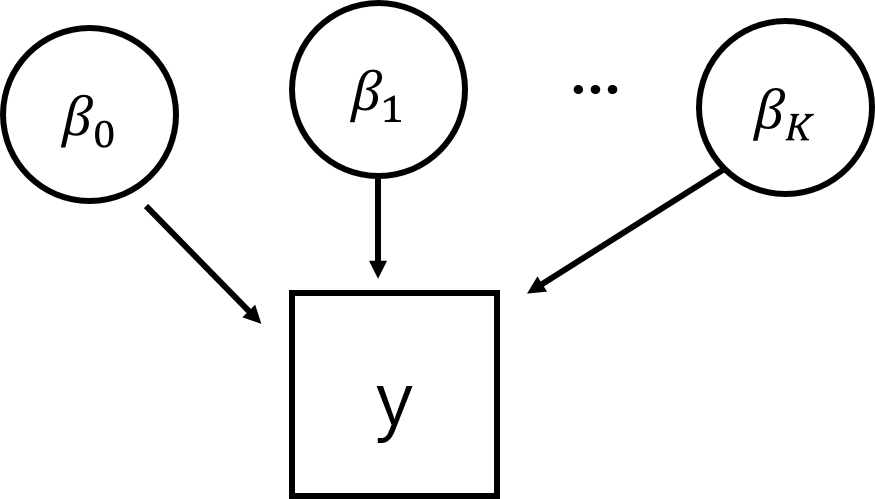
\includegraphics[scale=0.5]{regModel.png}
\end{figure}


\subsection{Model Proposal}

\begin{figure}[h!]
	\centering
	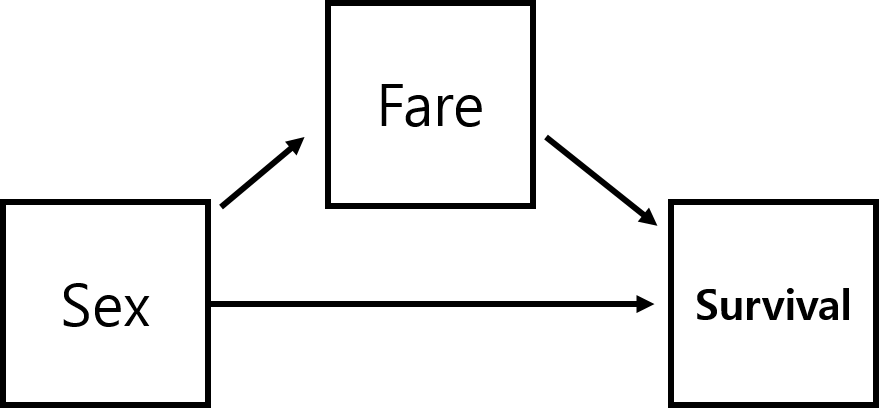
\includegraphics[scale=0.5]{titanicModel.png}
\end{figure}


$$
\begin{aligned}
X_{Sex} |\theta_{Sex} &\sim Bernoulli(\theta_{Sex}) \\[8pt]
X_{Fare} | \xi_{SexEffect}, \mu_{Fare}, \sigma_{Fare}, X_{Sex} &\sim LogNormal(\mu_{Fare} + \xi_{SexEffect} X_{Sex}, \sigma_{Fare}) \\[8pt]
X_{Survival} | \psi_{SexEffect}, \psi_{FareEffect} &\sim Bernoulli(\theta_{Survival} + \psi_{SexEffect} X_{Sex} + \psi_{FareEffect} X_{Fare})
\end{aligned}
$$



\end{document}